\documentclass[11pt,a4paper]{article}

% --- Encoding & fonts ---
\usepackage[utf8]{inputenc}
\usepackage[T1]{fontenc}
\usepackage{lmodern}

% --- Page geometry ---
\usepackage[margin=2.5cm]{geometry}

% --- Language ---
\usepackage[english]{babel}

% --- Graphics & figures ---
\usepackage{graphicx}
\graphicspath{{figures/}}
\usepackage{subcaption}   % side-by-side figures
\usepackage{float}        % [H] placement

% --- Tables ---
\usepackage{booktabs}
\usepackage{tabularx}
\usepackage{multirow}

% --- Math ---
\usepackage{amsmath,amssymb}

% --- Bibliography ---
\usepackage[backend=biber,style=authoryear,maxcitenames=2,natbib=true]{biblatex}
\addbibresource{references.bib}

% --- Hyperlinks & cross-references ---
\usepackage[colorlinks=true,linkcolor=blue!60!black,citecolor=green!50!black,urlcolor=blue!70!black]{hyperref}
\usepackage[capitalise,noabbrev]{cleveref}

% --- Code listings (optional, for appendix) ---
\usepackage{listings}
\lstset{basicstyle=\ttfamily\small,breaklines=true}

% --- Misc ---
\usepackage{xcolor}
\usepackage{enumitem}
\usepackage[section]{placeins}  % keep floats within their section

% --- Title ---
\title{GNN-SDM: Species Distribution Modelling with Graph Neural Networks for Swiss Flora at 30\,m Resolution}
\author{
  Kevin M\"uller \\
  \texttt{kevin.mueller@example.ch}
}
\date{\today}

% =============================================================================
\begin{document}

\maketitle
\thispagestyle{empty}

\begin{abstract}
Traditional species distribution models treat occurrences as independent points, ignoring the spatial structure of landscapes that governs habitat connectivity and species dispersal. We adapt the GNN-SDM framework \citep{Wu2025} to Swiss vascular plants at 30\,m resolution, constructing a landscape graph of 166,464 patches linked by 465,833 adjacency edges. Using a GraphSAGE architecture tuned for flora, we model habitat suitability for 3,751 species and compare against a Random Forest baseline. [Results summary to be added.]
\end{abstract}

\newpage
\tableofcontents
\newpage

% --- Sections in separate files for manageability ---
\section{Introduction}
\label{sec:introduction}

% --- Biodiversity loss and habitat fragmentation in Switzerland ---

Biodiversity is declining at an unprecedented rate worldwide, driven by habitat 
loss, fragmentation, climate change, and land-use intensification \citep{IPBES2019}. 
Switzerland, despite its relatively small area, harbours exceptional plant 
diversity owing to its pronounced altitudinal gradients and mosaic of biogeographic 
regions. Yet even here, a third of all assessed species and half of all habitat 
types are threatened \citep{FOEN2022}, with 28\% of vascular plants considered 
endangered or regionally extinct and an additional 14\% near-threatened 
\citep{InfoFlora2024}. The main drivers---soil sealing, landscape fragmentation, 
intensive land use, and nitrogen inputs---continue to erode habitat quality and 
connectivity \citep{FOEN2022,FOEN2025}. Effective conservation planning requires 
spatially explicit predictions of where species can persist, and crucially, which 
landscape elements link suitable habitat patches into functional networks.

% --- Traditional SDMs: strengths and limitations ---

Species distribution models (SDMs) have become a cornerstone of conservation 
biogeography, relating georeferenced occurrence records to environmental 
predictors to map habitat suitability across space \citep{Elith2009,Guisan2005}. 
Classical approaches, such as generalised linear models, maximum entropy \citep{Phillips2006}, 
and ensemble methods such as Random Forests \citep{Breiman2001}, treat each 
occurrence as an independent sample drawn from an environmental niche. While powerful, 
this point-based paradigm ignores the spatial structure of landscapes: two 
patches with identical environmental conditions may differ dramatically in 
ecological value depending on their size, shape, and connectivity to neighbouring 
habitat. For species whose long-term persistence depends on seed dispersal between 
habitat patches, such as the Cypripedium calceolus, this omission can lead to 
misleading suitability estimates and suboptimal conservation recommendations.

% --- GNN-SDM framework: how graph structure captures landscape interactions ---

Graph Neural Networks (GNNs) offer a principled way to incorporate landscape 
structure into SDMs. By representing the landscape as a graph, where nodes are 
ecologically homogeneous patches and edges encode spatial adjacency. A GNN can 
learn how environmental conditions in neighbouring patches jointly influence 
local habitat suitability. \citet{Wu2025} introduced the SOM-GNN-SDM framework, 
demonstrating that a GraphSAGE architecture \citep{Hamilton2017} trained on 
landscape graphs substantially outperforms traditional SDMs for virtual and real
species across continental extents. Their approach constructs landscape patches 
via Self-Organising Maps (SOMs) \citep{Kohonen1982}, builds an adjacency graph, 
and propagates information across the graph to produce suitability predictions 
that are spatially coherent and connectivity-aware.

% --- Conservation application: graph structure for gap identification ---

Beyond improving predictive accuracy, the graph representation opens a direct 
path to conservation applications. The Swiss federal government has identified 
the lack of an ecological infrastructure that protects and connects core 
biodiversity areas as a key deficit, setting a target of 17\% of national 
territory as connected core areas by 2030, up from 13.4\% today 
\citep{FOEN2022,FOEN2025}. Because the landscape graph explicitly encodes 
connectivity, it can be analysed using circuit theory and centrality metrics to 
identify critical corridors: patches whose protection would maintain or restore 
habitat connectivity for threatened species. This transforms the SDM output from 
a static suitability map into an actionable tool for spatial conservation 
prioritisation and gap analysis, directly informing where the ecological 
infrastructure should be expanded.

% --- Our contribution ---

In this work, we adapt the GNN-SDM framework to Swiss vascular flora at 30\,m 
resolution, presenting a substantially finer grain than the original continental-scale 
application. We construct a landscape graph of 166,464 patches from 12 environmental 
features using SOM-based clustering and connected-component labelling, train 
per-species GraphSAGE models for 3,751 qualifying plant species, and benchmark 
against a Random Forest baseline. We further apply circuit-theory connectivity 
analysis to the resulting suitability maps to identify conservation priority 
areas and quantify protection gaps relative to the existing protected-area network.

% --- Research questions ---

Specifically, we address the following research questions:
\begin{enumerate}[nosep]
  \item Can GNN-SDM outperform a traditional Random Forest at patch-level species distribution modelling for Swiss plants?
  \item Does the graph structure confer greater benefit for rare and vulnerable species, whose distributions are more fragmented?
  \item What GNN architecture is best suited for flora---given that plants, unlike the mobile fauna studied by \citet{Wu2025}, have limited active dispersal?
  \item Can the graph structure be leveraged to identify spatial gaps in the protected-area network where additional conservation measures would be most beneficial?
\end{enumerate}


\section{Data and Study Area}
\label{sec:data}

\subsection{Study Area}
\label{sec:study-area}

The study area encompasses the entirety of Switzerland and a surrounding buffer zone, defined by the spatial extent of the CHELSAch high-resolution climate dataset \citep{CHELSAch}. The bounding box spans from 45.57°\,N to 48.07°\,N latitude and 5.72°\,E to 10.66°\,E longitude, covering approximately 41,400\,km\textsuperscript{2} of land area. This extent includes a border buffer of roughly 10\,km into neighbouring countries to avoid edge effects in spatial analyses such as flow accumulation and neighbourhood-based feature computation.

All environmental layers are aligned to a common 30\,m master grid derived from the Copernicus GLO-30 Digital Elevation Model \citep{CopernicusDEM}, projected in geographic coordinates (EPSG:4326). Switzerland's topography ranges from 193\,m (Lake Maggiore) to 4,634\,m (Dufourspitze), creating steep environmental gradients over short distances---a property that motivates the use of high-resolution modelling.

\subsection{Environmental Features}
\label{sec:features}

We compiled 21 candidate environmental features from four thematic groups (\cref{tab:features}): terrain, land cover, climate, and biological/anthropogenic variables. All layers were processed to the 30\,m master grid using source-appropriate resampling methods.

\begin{table}[htbp]
\centering
\caption{Environmental predictor variables compiled for the study. All layers are aligned to the 30\,m master grid. The 12 features selected for modelling (after feature selection, \cref{sec:feature-selection}) are marked with~$\bullet$.}
\label{tab:features}
\small
\begin{tabularx}{\textwidth}{llXll}
\toprule
\textbf{Group} & \textbf{Feature} & \textbf{Source} & \textbf{Native res.} & \textbf{Sel.} \\
\midrule
\multirow{7}{*}{Terrain}
 & Elevation & Copernicus GLO-30 DEM & 30\,m & $\bullet$ \\
 & Slope & Derived from DEM & 30\,m & $\bullet$ \\
 & Aspect (sin, cos) & Derived from DEM & 30\,m & $\bullet$ \\
 & Topographic Wetness Index & D8 flow accumulation & 30\,m & $\bullet$ \\
 & Profile curvature & 2\textsuperscript{nd}-order finite diff. & 30\,m & \\
 & Plan curvature & 2\textsuperscript{nd}-order finite diff. & 30\,m & \\
\midrule
\multirow{6}{*}{Land cover}
 & Tree cover fraction & ESA WorldCover 2021 & 10\,m & $\bullet$ \\
 & Grassland fraction & ESA WorldCover 2021 & 10\,m & $\bullet$ \\
 & Cropland fraction & ESA WorldCover 2021 & 10\,m & $\bullet$ \\
 & Built-up fraction & ESA WorldCover 2021 & 10\,m & \\
 & Snow/ice fraction & ESA WorldCover 2021 & 10\,m & \\
 & Water fraction & ESA WorldCover 2021 & 10\,m & \\
\midrule
\multirow{5}{*}{Climate}
 & Bio1 (annual mean temp.) & CHELSAch & 25\,m & $\bullet$ \\
 & Bio4 (temp. seasonality) & CHELSAch & 25\,m & $\bullet$ \\
 & Bio12 (annual precip.) & CHELSAch & 25\,m & $\bullet$ \\
 & Bio15 (precip. seasonality) & CHELSAch & 25\,m & \\
 & Bio18 (precip. warmest quarter) & CHELSAch & 25\,m & \\
\midrule
\multirow{4}{*}{Biological}
 & Canopy height & ETH Global Canopy Height & 10\,m & $\bullet$ \\
 & NDVI (annual max) & GIMMS MODIS & 250\,m & \\
 & Human Footprint & \citet{Mu2022} & 1\,km & $\bullet$ \\
 & Forest-edge distance & Derived from tree cover & 30\,m & \\
\bottomrule
\end{tabularx}
\end{table}

\paragraph{Terrain features.}
Elevation was obtained directly from the Copernicus GLO-30 DEM \citep{CopernicusDEM}. Slope and aspect were derived using first-order finite differences at 30\,m resolution. Aspect was encoded as two variables (sin and cos of the azimuth angle) to avoid the circular discontinuity at 0°/360°. The Topographic Wetness Index (TWI) was computed using D8 flow direction and accumulation via the \texttt{pysheds} library, with pit-filling and depression resolution applied beforehand. Profile and plan curvature were derived from second-order finite differences and smoothed with a 5$\times$5 mean filter to reduce noise.

\paragraph{Land cover.}
Six land-cover fraction layers were computed from ESA WorldCover 2021 \citep{ESAWorldcover} at its native 10\,m resolution. For each class, a binary mask was reprojected to the 30\,m grid using average resampling, yielding the fraction of each 30\,m pixel covered by that land-cover type. The six classes retained for Switzerland are: tree cover, grassland, cropland, built-up, snow/ice, and permanent water bodies.

\paragraph{Climate.}
Five bioclimatic variables were derived from CHELSAch monthly temperature and precipitation normals (1981--2010) at 25\,m resolution \citep{CHELSAch}: annual mean temperature (Bio1), temperature seasonality (Bio4, standard deviation), annual precipitation (Bio12), precipitation seasonality (Bio15, coefficient of variation), and precipitation of the warmest quarter (Bio18). Each variable was regridded to the 30\,m master grid using bilinear interpolation.

\paragraph{Biological and anthropogenic features.}
Canopy height was obtained from the ETH Global Canopy Height Model at 10\,m resolution \citep{Lang2023} and regridded to 30\,m via bilinear resampling. The annual maximum NDVI was computed from GIMMS MODIS 8-day composites (250\,m, growing season DOY 97--273) and regridded to 30\,m. The global Human Footprint index \citep{Mu2022} at 1\,km was bilinearly downscaled. Forest-edge distance was computed as a signed Euclidean distance transform from the tree-cover fraction layer (threshold 0.5): positive values indicate distance from forest, negative values indicate depth within forest.

\subsection{Species Occurrence Data}
\label{sec:species-data}

Species occurrence records for vascular plants in Switzerland were obtained from the Global Biodiversity Information Facility (GBIF) open data snapshot hosted on Amazon S3 \citep{GBIF2024}. The raw dataset was filtered to retain only records within the study extent that met the following quality criteria: coordinate uncertainty $\leq$\,1000\,m, valid geographic coordinates, and taxonomic rank at species level.

After filtering, the dataset comprised approximately 14 million occurrence records spanning 7,912 vascular plant species. For modelling purposes, we retained only species with at least 100 unique occurrence records, yielding 3,756 qualifying species. This threshold ensures sufficient training data for both the Random Forest baseline and the GNN-SDM, while acknowledging that it excludes many rare and threatened species with sparse observational records.

% \begin{figure}[htbp]
%   \centering
%   \includegraphics[width=0.7\textwidth]{species_records_histogram.png}
%   \caption{Distribution of GBIF occurrence records per species (log scale). The dashed line indicates the 100-record threshold applied for model training.}
%   \label{fig:species-histogram}
% \end{figure}

\subsection{Protected Areas}
\label{sec:protected-areas}

Protected area boundaries for Switzerland were obtained from the World Database on Protected Areas (WDPA), filtered to nationally designated sites within the study extent. The dataset includes national parks, nature reserves, landscape protection areas, and Ramsar sites. These boundaries are used in the gap analysis (\cref{sec:gap-analysis}) to assess the degree to which high-priority habitat identified by the GNN-SDM falls within existing protected areas.

\subsection{Feature Selection}
\label{sec:feature-selection}

To reduce multicollinearity and computational cost, we performed feature selection using Random Forest importance scores. A patch-level RF classifier was trained for six representative species spanning different habitat types and prevalence levels. Feature importance was computed as the mean decrease in Gini impurity, averaged across species.

From the initial 21 candidate features, 12 were retained for downstream modelling (\cref{tab:features}). The excluded features were either highly correlated with retained variables (e.g., Bio15 with Bio12; plan curvature with profile curvature) or contributed negligible predictive power (e.g., NDVI at 250\,m resolution added little beyond the 10\,m canopy height and tree-cover fraction). The selected feature set balances ecological interpretability with predictive performance while keeping the dimensionality manageable for the Self-Organising Map clustering step.

% \begin{figure}[htbp]
%   \centering
%   \includegraphics[width=0.8\textwidth]{feature_importance_heatmap.png}
%   \caption{Random Forest feature importance (mean decrease in Gini impurity) for six representative species. Features below the dashed line were excluded from downstream modelling.}
%   \label{fig:feature-importance}
% \end{figure}

\section{Methods}
\label{sec:methods}

This section describes the methodological pipeline for constructing a graph-based 
species distribution model (SOM-GNN-SDM) for Swiss flora at 30\,m resolution, 
following the framework proposed by \citet{Wu2025}. The pipeline consists of three 
stages: 
landscape patch construction via Self-Organising Map clustering and connected-
component analysis, (2)~a Random Forest baseline, and (3)~the SOM-GNN-SDM itself.

\subsection{Landscape Patch Construction}
\label{sec:patches}

The landscape patch construction transforms the continuous 30\,m raster feature 
stack into a graph representation where nodes correspond to ecologically 
homogeneous habitat patches and edges encode spatial adjacency.

\subsubsection{SOM Clustering}
\label{sec:som}

A Self-Organising Map \citep[SOM;][]{Kohonen1982} was trained to identify 
recurring landscape types from the 12 selected environmental features. The SOM 
was configured as a $64 \times 64$ hexagonal, toroidal grid and initialised with 
PCA. Training used a subsample of 500\,000 pixels (drawn from the ${\sim}160$\,M
valid pixels in the study extent), preprocessed with a \texttt{RobustScaler} and 
domain-specific post-scaling (land-cover fractions up-weighted $3\times$; 
forest-edge distance clipped to $[-5, 5]$).

The SOM was trained for 150 epochs with a neighbourhood radius decaying from 64 
to 16 and a learning rate decaying from 0.05 to 0.016. Convergence was assessed 
on a held-out 20\% validation set using quantisation error (QE) and topographic 
error (TE).

After training, the codebook vectors were hierarchically clustered using Ward's 
linkage, and the dendrogram was cut to yield 30 landscape types. Every valid 
pixel in the study extent was then assigned to its best-matching unit (BMU) via 
a FAISS exact-$L_2$ index, producing a categorical landscape-type raster at 30\,
m resolution.

\subsubsection{Connected Components and Patch Merging}
\label{sec:components}

Spatially contiguous regions of the same landscape type were identified using 
connected-component labelling (\texttt{skimage.measure.label}). To avoid an 
excessive number of tiny fragments, patches smaller than 100 pixels 
(${\sim}0.09$\,km$^2$) were merged into their most similar neighbour using a 
mapping-table approach. This procedure yielded \textbf{166,464 landscape patches} 
covering the full study extent.

For each patch, the mean value of the 12 selected environmental features was 
computed from the underlying raster stack, producing a $166{,}464 \times 12$ 
node-feature matrix.

\subsubsection{Patch Network}
\label{sec:network}

An undirected graph was constructed by connecting patches that share at least 
one boundary pixel. The resulting \texttt{NetworkX} graph contains 
\textbf{166,464 nodes} and \textbf{465,833 edges}. Node attributes are the mean 
environmental features; no edge weights were used.

\subsection{Baseline: Random Forest}
\label{sec:rf}

A per-species Random Forest \citep{Breiman2001} classifier served
as the non-spatial baseline. For each of the 2,696 qualifying
species ($\geq 20$ presence patches), the following procedure was
applied:

\begin{enumerate}
    \item \textbf{Presence labels.} GBIF occurrence coordinates were mapped to 
    the patch-label raster, yielding a set of presence patches per species.
    \item \textbf{Pseudo-absence generation.} Background patches were sampled at 
    a 3:1 ratio (absence\,:\,presence) from patches without recorded occurrences, 
    using a fixed random seed for reproducibility.
    \item \textbf{Model training.} A \texttt{scikit-learn} Random Forest 
    was trained on the patch-level mean features using tuned hyperparameters 
    (see below).
    \item \textbf{Evaluation.} Performance was assessed via 5-fold cross-validated 
    metrics: AUC, accuracy, precision, recall, F1, MCC, Cohen's $\kappa$, and TSS.
\end{enumerate}

Hyperparameter tuning was performed via \texttt{GridSearchCV} on the same 
six representative species used for the GNN architecture search, covering 
diverse habitat types across Switzerland. The best hyperparameters from 
this limited tuning were then applied uniformly to all
2,696 species.

\subsection{GNN-SDM}
\label{sec:gnn}

\subsubsection{Model Architecture}
\label{sec:architecture}

The SOM-GNN-SDM is based on GraphSAGE \citep{Hamilton2017}, implemented in 
PyTorch Geometric \citep{Fey2019}. At each layer $l$, a node $v$ aggregates 
information from its neighbourhood $\mathcal{N}(v)$ using the mean aggregator 
and combines it with its own representation:
\begin{align}
    \mathbf{h}^{(l)}_{\mathcal{N}(v)} &= \frac{1}{|\mathcal{N}(v)|} 
        \sum_{u \in \mathcal{N}(v)} \mathbf{h}^{(l-1)}_u 
        \label{eq:sage-agg} \\
    \mathbf{h}^{(l)}_v &= \sigma\!\left( 
        \mathbf{W}^{(l)} \cdot 
        \mathrm{CONCAT}\!\left( 
            \mathbf{h}^{(l-1)}_v,\; 
            \mathbf{h}^{(l)}_{\mathcal{N}(v)} 
        \right) 
    \right) \label{eq:sage-update}
\end{align}
where $\mathbf{h}^{(0)}_v = \mathbf{x}_v$ is the input feature vector of 
node $v$, $\mathbf{W}^{(l)}$ is a learnable weight matrix, and $\sigma$ is 
the LeakyReLU activation function. Dropout ($p = 0.2$) is applied after each 
layer during training. The final node embeddings are passed through a linear 
layer with sigmoid activation to produce a habitat-suitability score 
$\hat{y}_v \in [0, 1]$ for every patch:
\begin{equation}
    \hat{y}_v = \mathrm{sigmoid}\!\left( 
        \mathbf{w}^\top \mathbf{h}^{(L)}_v + b 
    \right) \label{eq:sage-output}
\end{equation}
where $L$ is the number of GraphSAGE layers.

An architecture search was conducted on six representative species spanning 
diverse habitats (\textit{Picea abies}, \textit{Fagus sylvatica}, 
\textit{Trifolium pratense}, \textit{Potentilla erecta}, 
\textit{Phragmites australis}, \textit{Senecio inaequidens}). 
Six architectures were compared:

\begin{itemize}
    \item 1-layer: $[16]$ (417 parameters)
    \item 2-layer: $[24, 12]$ (1,201 parameters)
    \item Paper default: $[24, 18, 8]$ (1,787 parameters)
    \item Wider: $[48, 32, 16]$ (5,361 parameters)
    \item Extra-wide: $[64, 48, 32]$ (10,929 parameters)
    \item 4-layer: $[32, 24, 16, 8]$ (3,417 parameters)
\end{itemize}

The extra-wide 3-layer architecture $[64, 48, 32]$ consistently achieved the 
highest mean AUC across all test species and was selected for production training. 
This is notably wider than the $[24, 18, 8]$ architecture proposed by \citet{Wu2025} 
for virtual fauna species, suggesting that flora---with their sessile nature and 
finer-grained habitat associations---benefit from greater representational 
capacity per layer rather than additional depth.

\subsubsection{Training Procedure}
\label{sec:training}

For each species, the GNN-SDM was trained independently using the following pipeline:

\begin{enumerate}
    \item \textbf{Background selection via random pseudo-absence.}
    Non-presence patches were sampled at a 3:1 ratio (background\,:\,presence) 
    using a fixed random seed. An initial design based on One-Class SVM background 
    selection \citep[as in][]{Wu2025} was evaluated during development but 
    abandoned in favour of random pseudo-absence for the production run. The 
    random strategy ensures a fair comparison with the RF baseline (which uses 
    same pseudo-absence protocol) and proved more robust across the full species 
    set, avoiding the computational overhead and occasional instability of 
    fitting a kernel SVM on high-dimensional patch features for
    each of 2,696 species.

    \item \textbf{PageRank weighting.}
    Presence patches were weighted by their PageRank centrality in the landscape 
    graph, following \citet{Wu2025}. This assigns higher importance to 
    structurally well-connected patches, reflecting their greater ecological 
    significance as habitat corridors or core areas. Background patches received 
    uniform weight of 1.0.

    \item \textbf{Train/validation split.}
    The labelled patches (presence $+$ background) were shuffled and split 80/20 
    into training and validation sets.

    \item \textbf{Optimisation.}
    The model was trained with the Adam optimiser (learning rate $= 0.001$) 
    using a weighted mean-squared-error loss:
    \[
        \mathcal{L} = \frac{1}{|\mathcal{T}|} \sum_{i \in \mathcal{T}} w_i \left( \hat{y}_i - y_i \right)^2
    \]
    where $\mathcal{T}$ is the training set, $w_i$ the PageRank-derived weight, 
    $\hat{y}_i$ the predicted suitability, and $y_i \in \{0, 1\}$ the label.

    \item \textbf{Early stopping.}
    Validation AUC was evaluated every 10 epochs. Training was halted if no 
    improvement occurred for 50 consecutive epochs (patience). The model state 
    with the best validation AUC was restored for prediction. Maximum training 
    duration was 500 epochs.

    \item \textbf{Prediction.}
    The best model was used to predict habitat suitability for all 166,464 
    patches, yielding a continuous suitability surface per species.
\end{enumerate}

\subsubsection{Evaluation}
\label{sec:evaluation}

To evaluate the GNN-SDM on the same footing as the RF baseline, a post-hoc 
evaluation was performed for each species: presence patches and a 3:1 random 
sample of non-presence patches were combined, and the predicted suitability 
scores were evaluated using the same eight metrics (AUC, accuracy, precision, 
recall, F1, MCC, Cohen's $\kappa$, TSS) with a classification threshold of 0.5.

\subsubsection{Computational Setup}
\label{sec:compute}

Production training of all 2,696 species was executed as an AWS
SageMaker Training Job on a GPU instance (NVIDIA GPU,
CUDA-accelerated). The job supported checkpointing for
spot-instance interruptions and completed in approximately 5.7
hours of GPU time (mean 7.6\,s per species, 231 epochs on
average). Node features were standardised (zero mean, unit variance) 
before training, and the full graph (166,464 nodes, 931,666 directed edges) was 
loaded onto the GPU for efficient message passing.

\subsection{Conservation Prioritisation}
\label{sec:conservation}

The final stage of the pipeline combines the GNN-SDM habitat suitability 
predictions with circuit-theory connectivity analysis to produce a multi-species 
conservation priority surface, which is then overlaid with existing protected 
areas to identify protection gaps.

\subsubsection{Complementarity of Suitability and Connectivity}
\label{sec:complementarity}

One might ask whether the circuit-theory step is redundant 
given that GraphSAGE already incorporates neighbourhood information during 
message passing. The two components are, however, fundamentally complementary:

\begin{itemize}
    \item \textbf{GNN suitability} is a \emph{local} property. GraphSAGE 
    aggregates features from the 1--2 hop neighbourhood to predict whether a 
    given patch is suitable habitat for a species. The output answers: 
    ``Is this place good habitat?''

    \item \textbf{Circuit-theory current flow} is a \emph{global network} 
    property. It treats the entire landscape graph as an electrical circuit 
    and computes which patches act as irreplaceable bridges between isolated 
    population clusters. The output answers: ``Is this place critical for 
    maintaining connectivity between populations?''
\end{itemize}

These two perspectives are orthogonal. A patch may have moderate suitability 
(GNN score ${\sim}0.3$) yet carry very high current because it lies in the only 
traversable corridor between two populations. Conversely, a patch in the core 
of a large population may have high suitability but low current because 
alternative paths exist. The highest conservation value lies a patches that score
highly on both dimensions.

\subsubsection{Circuit-Theory Connectivity}
\label{sec:circuit}

For each species, the landscape graph is treated as a resistor network where 
the conductance of each edge $(u, v)$ is defined as the mean suitability of 
the two adjacent patches:
\begin{equation}
    g_{uv} = \max\!\left( 10^{-4},\; 
        \frac{\hat{y}_u + \hat{y}_v}{2} 
    \right)
    \label{eq:conductance}
\end{equation}
This ensures that current preferentially flows through high-suitability regions 
(low resistance), reflecting the ecological principle that organisms move more 
easily through suitable habitat.

Source and ground nodes are defined by the species' actual observation patches. 
These patches are grouped into connected components in the landscape graph; 
components with $\geq 3$ patches are ranked by size, and current flow is solved 
between the top $k = 6$ component pairs using Kirchhoff's circuit laws. 
Specifically, for each source--ground pair, one unit of current is injected 
uniformly across source nodes and extracted uniformly at ground nodes. The 
resulting system of linear equations (conductance Laplacian) is solved for node 
voltages using a sparse direct solver (\texttt{scipy.sparse.linalg.spsolve}), 
and the absolute current through each node is accumulated across all pairs.

Species with fewer than 2 qualifying components are excluded, as connectivity 
cannot be meaningfully assessed.

\subsubsection{Species Selection and Filtering}
\label{sec:species-selection}

The gap analysis targets nationally threatened species according
to the Swiss Red Lists of vascular plants
\citep{InfoFlora2016} and bryophytes \citep{InfoFlora2022},
published by Info Flora on behalf of BAFU (Federal Office for
the Environment). These lists apply IUCN criteria at the
\emph{national} level, as a species can be globally Least Concern
yet nationally Critically Endangered in Switzerland. 

Of the 2,696 GNN-trained species, 489 carry a nationally
threatened status (CR, EN, VU, or NT). Two additional filters
are applied:

\begin{enumerate}
    \item \textbf{Minimum spatial structure.} Only species with
    $\geq 50$ presence patches are retained, ensuring sufficient
    spatial extent for meaningful circuit-theory analysis. This
    yields \textbf{285 species} (CR\,=\,2, EN\,=\,20, VU\,=\,93,
    NT\,=\,170).

    \item \textbf{Minimum connectivity.} During computation,
    species whose observation patches form fewer than 2 connected
    components of size $\geq 3$ are excluded, as the
    circuit-theory framework requires at least one
    source--ground pair. This removes a further 44 species,
    leaving 241 species with non-zero current flow.
\end{enumerate}

\subsubsection{Normalisation and Aggregation}
\label{sec:aggregation}

Per-species current flow values span vastly different scales
depending on graph structure and population fragmentation. To
ensure each species contributes on a comparable scale to the
multi-species aggregation, each species' current vector is
mean-normalised:
\begin{equation}
    \tilde{c}_{v} = \frac{c_v}{\bar{c}}
    \label{eq:normalisation}
\end{equation}
where $\bar{c} = \frac{1}{N}\sum_{v} c_v$ is the species-level
mean current. Values are thus expressed as multiples of the
species mean: $\tilde{c}_v = 1$ indicates average flow, while
$\tilde{c}_v \gg 1$ identifies critical pinch-points. This
allows comparison across species whose absolute current
magnitudes differ: a species with many observed
patches generates higher raw current than one with few
observations, yet both may contain equally important
bottlenecks. Mean normalisation preserves the relative
importance of pinch-points within each species while placing
all species on a common scale. Species whose mean current is
effectively zero ($\bar{c} < 10^{-12}$) are excluded, leaving
241 of 285 species with non-zero flow.

Species are weighted by national Red List category
(CR\,=\,4, EN\,=\,3, VU\,=\,2, NT\,=\,1) to reflect
conservation urgency. The multi-species priority surface
is then computed as:
\begin{equation}
    P_v = \frac{1}{2}\left( 
        \frac{\sum_s w_s \hat{y}_{v,s}}{\sum_s w_s} + 
        \frac{\sum_s w_s \tilde{c}_{v,s}}{\sum_s w_s} 
    \right)
    \label{eq:priority}
\end{equation}
where $w_s$ is the threat-category weight of species $s$,
$\hat{y}_{v,s}$ the GNN suitability, and $\tilde{c}_{v,s}$
the normalised current flow at patch $v$.

\subsubsection{Protected Area Overlay}
\label{sec:overlay}

The Swiss protected area network (WDPA; 10,522 polygons) is rasterised onto 
the 30\,m patch grid. Each patch is assigned the fraction of its constituent 
pixels that fall within any protected area polygon. The analysis is restricted 
to patches within Swiss territory (majority of pixels inside the national 
boundary) to avoid false negatives from neighbouring countries.

Conservation gaps are quantified by examining what fraction of high-priority 
patches (top 5\% and top 10\% of the priority surface) currently lack any 
protected-area coverage. These unprotected high-priority patches represent 
the most urgent candidates for protection expansion.

\section{Results and Discussion}
\label{sec:results}

\subsection{Landscape Graph Construction}
\label{sec:som-results}

The SOM converged after approximately 150 training epochs on the
400\,000-pixel subsample (80\,\% of 500\,000, with 20\,\% held out
for validation). \Cref{fig:som-convergence} shows the evolution of
validation quantisation error (QE) and topographic error (TE) across
training stages. QE decreases monotonically throughout training,
but the codebook feature maps
(\cref{fig:codebook-comparison}) reveal that this continued
improvement comes at a cost: at 150~epochs, the codebook displays
smooth gradients with distinct regional structure, whereas at
200~epochs the features fragment into noise as the shrinking
neighbourhood radius causes individual neurons to overfit local
samples. While QE continues to decrease beyond 150~epochs, the
topographic error increases and the codebook loses the spatial
coherence needed for meaningful landscape-type clustering. The
final validation metrics (QE\,=\,1.54, TE\,=\,0.14) at 150~epochs
thus represent the best trade-off between quantisation fidelity and
topological preservation.

\begin{figure}[htbp]
  \centering
  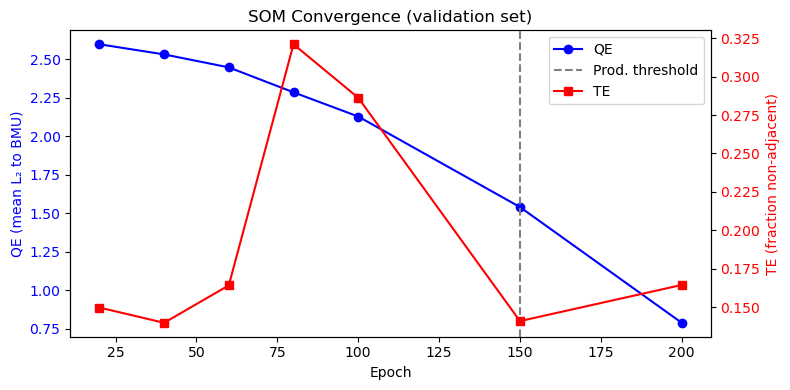
\includegraphics[width=0.75\linewidth]{som_convergence}
  \caption{SOM convergence on the held-out validation set. Left
  axis: quantisation error (mean $L_2$ distance to best-matching
  unit). Right axis: topographic error (fraction of samples whose
  two closest BMUs are non-adjacent on the grid). The dashed
  vertical line marks the 150-epoch production threshold.}
  \label{fig:som-convergence}
\end{figure}

Hierarchical clustering of the 4\,096 codebook vectors (Ward's
linkage, cut at 30 clusters) partitioned the SOM grid into 30
landscape types representing recurring environmental configurations
across Switzerland. Connected-component labelling and merging of
fragments smaller than 100~pixels produced the final landscape graph
of \textbf{166\,464 patches} and \textbf{465\,833 edges}.

The patch size distribution (\cref{fig:patch-stats}) shows a median
of 340~pixels (${\sim}0.31$\,km$^2$), with a long tail towards
larger contiguous patches in homogeneous terrain (e.g.\ alpine
grassland, dense forest). The minimum enforced size of 100~pixels
(${\sim}0.09$\,km$^2$) ensures that each patch is large enough to
carry ecologically meaningful feature averages.

The full-extent PCA-coloured patch map (\cref{fig:pca-patches}) reveals
coherent biogeographic structure: similar colours emerge for the
Swiss Plateau and the Po Valley south of the Alps, reflecting
analogous lowland environmental profiles. High-alpine zones form a
distinct cluster, while the southern Pre-Alps and Ticino group with
the Jura arc, both of which are characterised by their southward slope and
intermediate elevations.

\Cref{fig:landscape-roi} zooms into a ${\sim}16 \times 16$\,km
region north of Bern. Urban patches (Bern city centre) are clearly
delineated. The Dählhölzli forest along the Aare, the Schärmenwald
near Ittigen, and the Tiefenau peninsula emerge as distinct
forest-type patches. Overall, when compared with local knowledge,
clear ecological structures are visible at this resolution.

\begin{figure}[htbp]
  \centering
  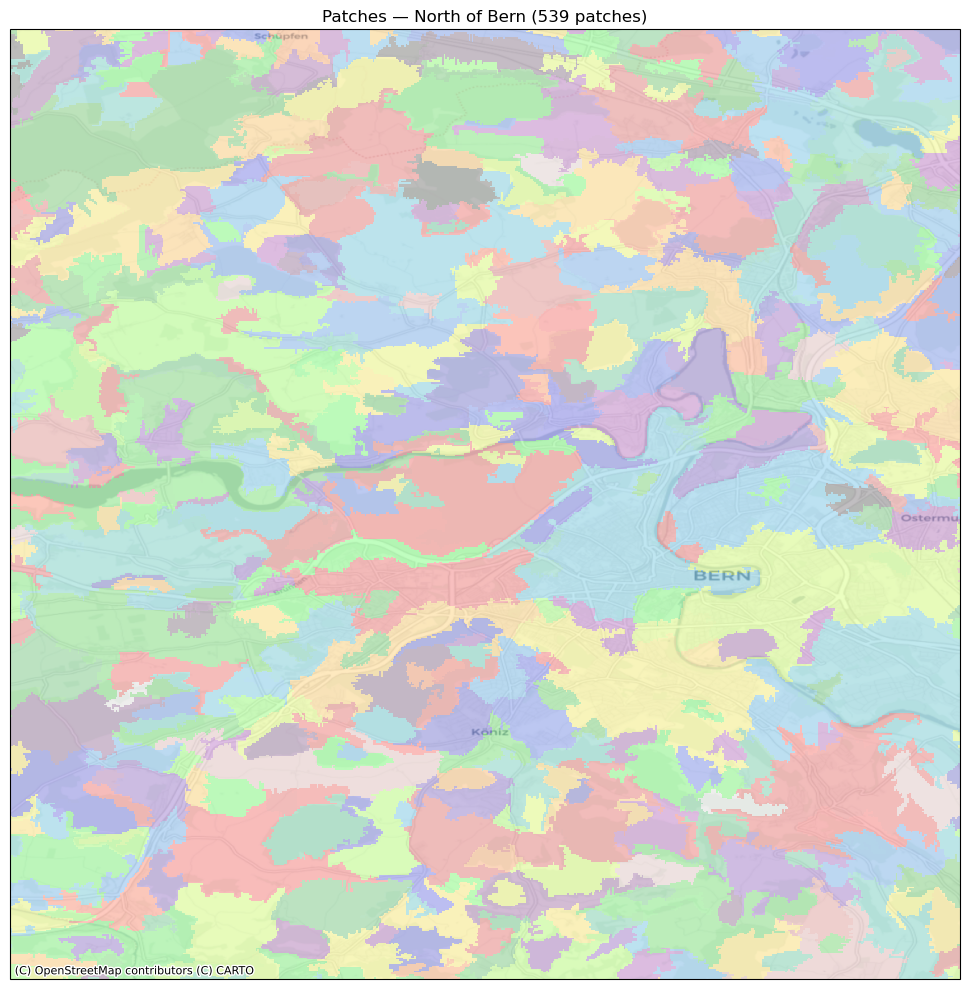
\includegraphics[width=0.85\linewidth]{patches_bern}
  \caption{Landscape-type map for the Bern region. Colours
  represent the 30 landscape types derived from hierarchical
  clustering of the SOM codebook. The tessellation captures
  transitions between forested hillsides, agricultural plains,
  and built-up areas at 30\,m resolution.}
  \label{fig:landscape-roi}
\end{figure}

\paragraph{Discussion.}
The SOM-based discretisation serves a dual purpose: it reduces the
${\sim}$160~million valid pixels to a tractable graph of 166\,464
nodes while ensuring that patch boundaries follow ecological
gradients rather than an arbitrary regular grid. This adaptive
resolution means that patches are smaller in heterogeneous landscapes
(e.g.\ valley floors with interspersed land cover) and larger in
homogeneous terrain (e.g.\ high-alpine meadows), mirroring the
spatial structure relevant to species distributions.

A limitation of the adjacency-based edge construction is that
connections between patches sharing only a single boundary pixel
receive the same weight as connections along extensive shared
borders. The graph therefore contains ``bridge'' edges representing
tenuous spatial contact (e.g.\ two forest patches touching through a
one-pixel corridor under a road). This is revisited in
\cref{sec:limit-detail}.

\subsection{Random Forest Baseline}
\label{sec:rf-results}

A per-species Random Forest served as the non-spatial baseline.
Across 3\,751 species, the RF achieved a mean AUC of 0.838
(median\,=\,0.834), with 99.4\,\% of species exceeding 0.7. Full
metric summaries are provided in \cref{app:rf-baseline}. The RF's
key limitation is its independence assumption: each patch is
classified without regard to its landscape context, so the model
cannot distinguish isolated habitat fragments from patches embedded
in connected corridors.

\subsection{Architecture Search}
\label{sec:arch-results}

Six GraphSAGE architectures were evaluated on six
representative species spanning a range of habitats and
prevalence levels (\cref{tab:arch-search}).  Performance was
measured by validation AUC averaged over the six species.

\begin{table}[htbp]
  \centering
  \caption{Architecture search results (validation AUC). Each
  column corresponds to one of the six representative species;
  the final column reports the mean across species.}
  \label{tab:arch-search}
  \small
  \begin{tabular}{lcccccc|c}
    \toprule
    Architecture & \textit{P.~ab.} & \textit{F.~sy.}
      & \textit{T.~pr.} & \textit{P.~er.}
      & \textit{Ph.~au.} & \textit{S.~in.} & Mean \\
    \midrule
    1-layer {[}16{]}        & 0.730 & 0.755 & 0.670
      & 0.700 & 0.734 & 0.877 & 0.744 \\
    2-layer {[}24,12{]}     & 0.742 & 0.785 & 0.715
      & 0.725 & 0.746 & 0.885 & 0.766 \\
    paper {[}24,18,8{]}     & 0.770 & 0.791 & 0.726
      & 0.751 & 0.771 & 0.901 & 0.785 \\
    wider {[}48,32,16{]}    & 0.791 & 0.807 & 0.752
      & 0.766 & 0.791 & 0.908 & 0.803 \\
    extra-wide {[}64,48,32{]} & 0.796 & 0.817 & 0.759
      & 0.776 & 0.794 & 0.911 & 0.809 \\
    4-layer {[}32,24,16,8{]} & 0.787 & 0.796 & 0.742
      & 0.750 & 0.776 & 0.906 & 0.793 \\
    \bottomrule
  \end{tabular}
\end{table}

The extra-wide architecture ({[}64,48,32{]}, 3~layers) yielded the
highest mean AUC (0.809) and was selected for all subsequent
experiments.  Adding a fourth layer did not improve performance,
suggesting that three message-passing hops (covering a
${\sim}$3-patch spatial neighbourhood) capture the relevant
landscape context for Swiss plant species.  This contrasts with
the original \cite{Wu2025} configuration ({[}24,18,8{]}),
which was optimised for global-scale fauna; wider hidden layers
appear necessary to capture the finer environmental gradients
that distinguish Swiss vegetation zones at 30\,m resolution.

\paragraph{Graph structure benefit.}
The improvement from one to three GraphSAGE layers quantifies how
much each species profits from neighbourhood information
propagated through the landscape graph. The largest gains are
observed for alpine and subalpine grassland species---notably
\textit{Potentilla erecta} ($+0.051$ AUC) and \textit{Trifolium
pratense} ($+0.056$)---while the habitat specialist
\textit{Senecio inaequidens} benefits least ($+0.024$), as its
distinct urban niche is already well captured by local features
alone.

\textit{Potentilla erecta} (alpine grassland) provides a
particularly clear illustration. This species occupies connected
subalpine meadow patches in distinct elevation bands, shaped by
climate and topography rather than human management. With a
single GraphSAGE layer, predictions rely solely on local patch
features; isolated meadow patches receive unreliable scores
because the model lacks spatial context. With three layers, the
GNN propagates suitability information through adjacent patches,
correctly identifying connected alpine grassland belts as
suitable habitat---even where direct observations are absent.
This spatial smoothing through the graph is the core mechanism
by which SOM-GNN-SDM surpasses the non-spatial RF baseline for
spatially structured species (see \cref{sec:gnn-results}).

\subsection{SOM-GNN-SDM Performance}
\label{sec:gnn-results}

% Same metrics, GNN vs RF comparison
% Where does graph structure help?
% Where does RF suffice (generalists)?

\textbf{TODO: GNN results and comparison with RF.}


\subsection{Common vs.\ Vulnerable Species}
\label{sec:species-comparison}

% Deep dive on 12 species (6 common + 6 vulnerable)
% Overprediction discussion: sampling bias, SDM purpose
% Specialists vs generalists performance difference

\textbf{TODO: Species-level analysis.}

\subsection{Habitat Suitability Maps}
\label{sec:maps}

% Example maps for selected species
% Visual validation against known ranges

\textbf{TODO: Map figures.}

\subsection{Conservation Prioritisation}
\label{sec:conservation-results}

% Circuit-theory connectivity results
% Gap analysis: priority areas vs protected areas
% Quantification of conservation gaps

\textbf{TODO: Conservation application results.}

\section{Limitations and Future Work}
\label{sec:limitations}

\subsection{Limitations}
\label{sec:limit-detail}

% Resolution vs computational cost
% GBIF sampling bias (spatial, temporal, taxonomic)
% Temporal snapshot — no climate change projection
% No independent field validation
% Single-pixel connections: no edge weighting by
%   corridor width or resistance
% SOM quantisation loss

\textbf{TODO: Limitations.}

\subsection{Future Directions}
\label{sec:future}

% Multi-species GNN (joint embedding)
% Temporal dynamics / climate scenarios
% Transfer learning to other regions
% Edge-weighted graph (resistance surfaces)
% Lower occurrence threshold for rare species

\textbf{TODO: Future directions.}

\section{Conclusion}
\label{sec:conclusion}

Graph neural networks can effectively model habitat suitability for Swiss 
flora at 30\,m resolution. By encoding the landscape as a graph of
166,464 ecologically homogeneous patches linked by spatial
adjacency, the SOM-GNN-SDM framework captures spatial context
that traditional per-site models cannot represent.

Three main results:

\begin{enumerate}
  \item \textbf{Graph structure improves predictions.} The
    GNN-SDM outperforms the Random Forest baseline for
    85.3\,\% of 2,696 species (mean AUC 0.912 vs 0.874,
    mean TSS 0.583 vs 0.430), with the largest gains for
    species whose distributions depend on landscape
    connectivity rather than local features alone.

  \item \textbf{The model generalises to rare species.}
    Nationally threatened species achieve comparable or
    higher discrimination (AUC 0.874, TSS 0.708) than
    common species, confirming that the framework is
    suitable for conservation applications despite lower
    observation density.

  \item \textbf{Significant protection gaps exist.}
    Circuit-theory connectivity analysis across 241
    threatened species reveals that 41\,\% of
    high-priority habitat patches---locations that are both
    suitable habitat and critical connectivity
    corridors---currently lack any formal protection.
\end{enumerate}

These results should be interpreted as a methodological
proof-of-concept rather than a direct policy recommendation.
Conservation decisions involve many factors beyond ecology:
a landscape patch identified as a critical ecological corridor
may simultaneously be productive farmland, infrastructure, or
subject to competing land-use interests. The priority surface
identifies \emph{where} ecological connectivity is most
vulnerable, but the question of \emph{whether} and \emph{how}
to act requires integration with socio-economic constraints,
stakeholder consultation, and on-the-ground verification that
lie beyond the scope of this analysis.

The full pipeline---from raw satellite and climate data to
actionable conservation priority maps---runs end-to-end in
under 10 hours of compute time and is readily transferable to
other regions or taxa. As Switzerland continues to develop its
ecological infrastructure strategy, data-driven approaches like SOM-GNN-SDM 
can complement expert assessment and field surveys with spatially explicit, 
reproducible evidence.

\section*{Acknowledgements}

This work was conducted as part of the Certificate of Advanced
Studies in Applied Machine Learning at the University of Bern. 
Computational resources (AWS SageMaker GPU
instances) were provided by the Federal Office for the
Environment (FOEN).

This report does not constitute a policy recommendation of the
FOEN. While the author is employed at FOEN and the programme
was partially funded by FOEN, this work was carried out
independently as an academic case study exploring the
application of machine learning to conservation planning. Any
interpretation of results in a policy context would require
additional validation, stakeholder engagement, and integration
with existing planning instruments.

AI assistance was used in the creation of this report as well
as in the creation of the code used.

\paragraph{Code availability.}
The full analysis pipeline (notebooks 00--32) is available at
\url{https://github.com/kronmar-bafu/cas-aml-project}.


% --- References ---
\newpage
\printbibliography

% --- Appendix (optional) ---
% \appendix
% \section{Supplementary Figures}
\label{app:figures}

\begin{figure}[htbp]
  \centering
  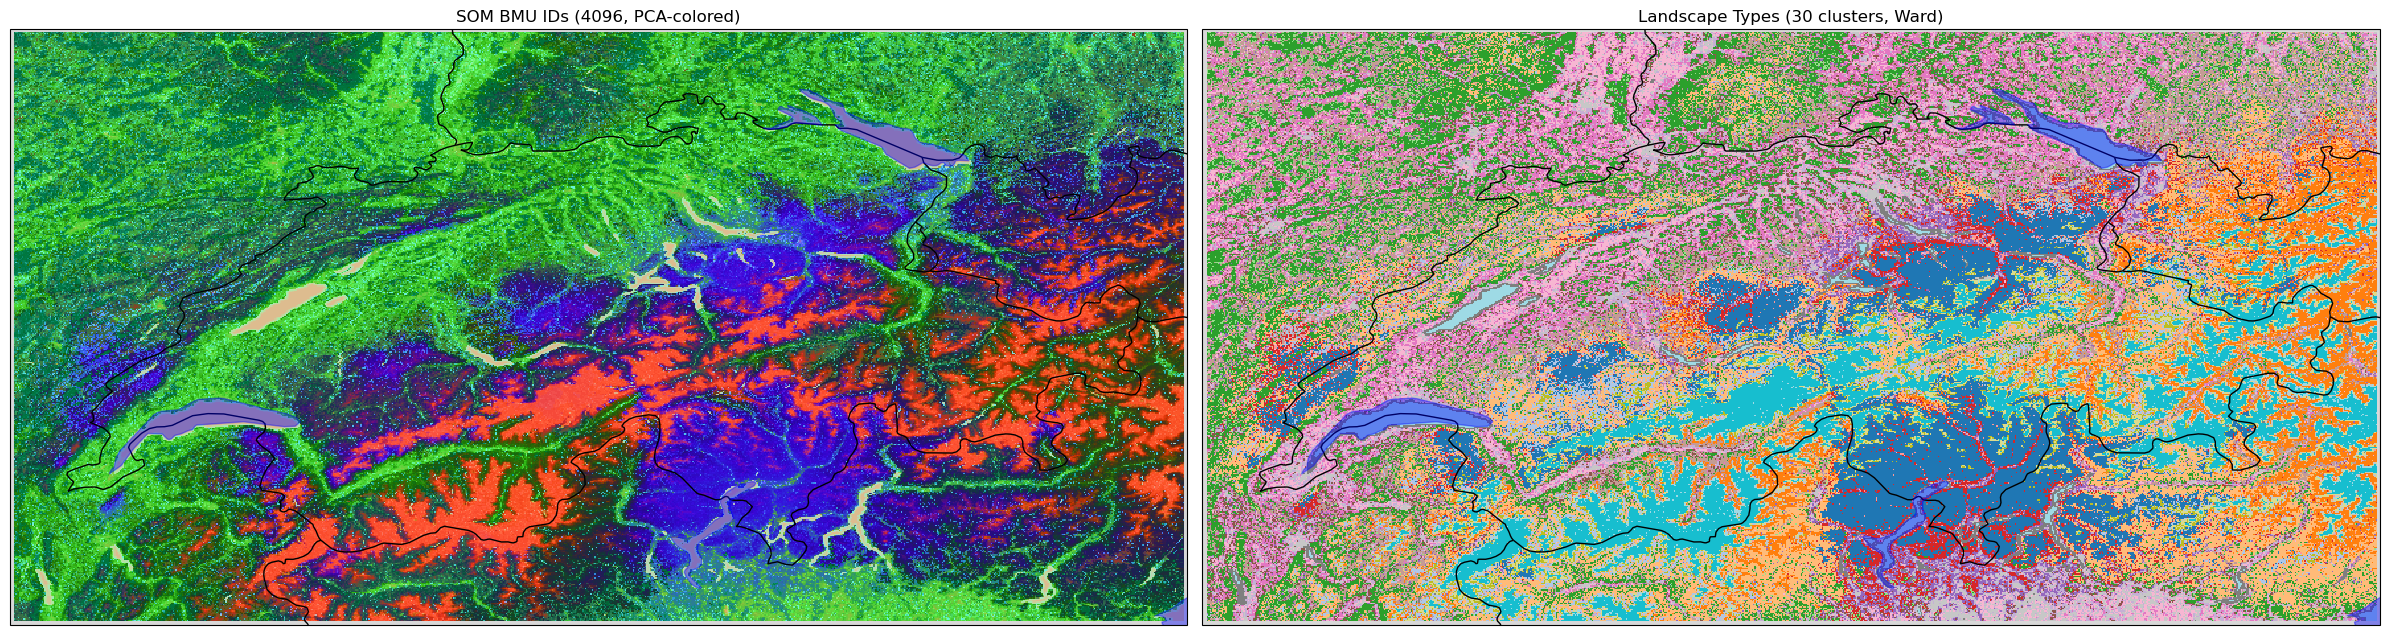
\includegraphics[width=\linewidth]{SOM_swiss}
  \caption{PCA-coloured landscape patch map of Switzerland.
  Codebook vectors are projected onto 3 principal components
  (mapped to RGB), so perceptually similar colours indicate
  environmentally similar patches. Major biogeographic zones
  are clearly distinguishable: lowland plateaus (Swiss Plateau,
  Po Valley) share warm tones, high-alpine areas appear as a
  distinct cool cluster, and forested pre-alpine slopes form
  intermediate gradients.}
  \label{fig:pca-patches}
\end{figure}

\begin{figure}[htbp]
  \centering
  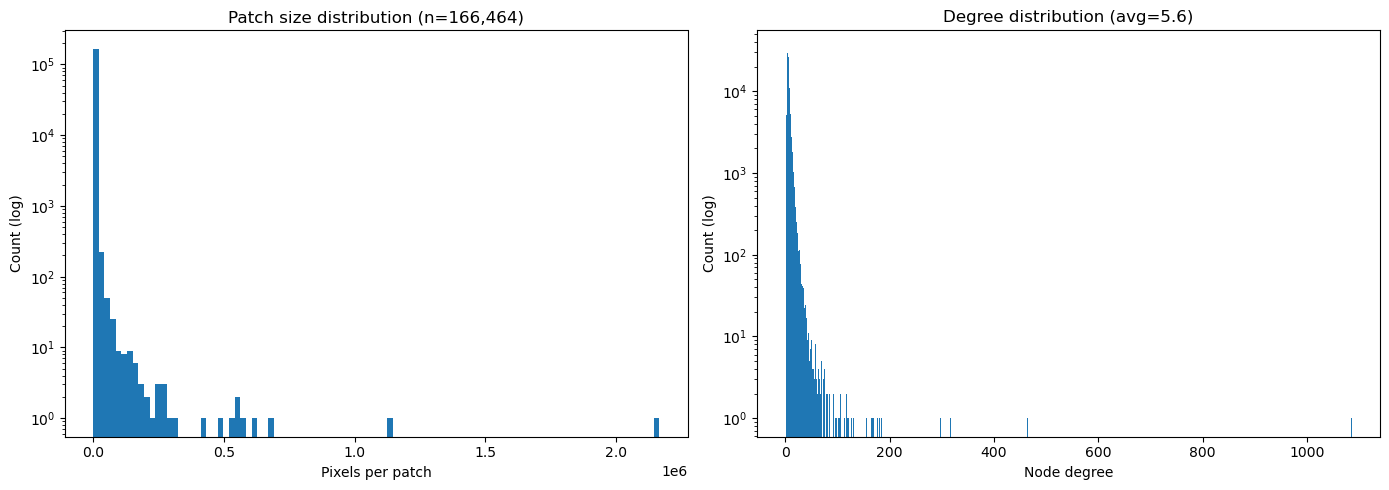
\includegraphics[width=0.8\linewidth]{patch_size_distribution}
  \caption{Patch size distribution (log scale) for the 166\,464
  landscape patches. The vertical dashed line marks the minimum
  threshold of 100~pixels (${\sim}0.09$\,km$^2$).}
  \label{fig:patch-stats}
\end{figure}

% Additional supplementary figures below this line

\section{Random Forest Baseline Details}
\label{app:rf-baseline}

\Cref{tab:rf-summary} summarises the cross-validated performance
metrics for the Random Forest baseline across all 2,696 species.

\begin{table}[htbp]
  \centering
  \caption{Random Forest baseline: summary statistics across
  2,696 species (5-fold cross-validation, threshold\,=\,0.5).}
  \label{tab:rf-summary}
  \begin{tabular}{lrrr}
    \toprule
    Metric & Mean & Median & Std \\
    \midrule
    AUC       & 0.874 & 0.877 & 0.056 \\
    Accuracy  & 0.832 & 0.831 & 0.042 \\
    Precision & 0.733 & 0.754 & 0.151 \\
    Recall    & 0.481 & 0.486 & 0.185 \\
    F1        & 0.561 & 0.585 & 0.173 \\
    MCC       & 0.498 & 0.512 & 0.163 \\
    TSS       & 0.430 & 0.433 & 0.176 \\
    \bottomrule
  \end{tabular}
\end{table}

The AUC distribution is strongly right-concentrated: 99.3\,\% of
species achieve AUC\,$>$\,0.7, and 91.6\,\% exceed 0.8.

\begin{figure}[htbp]
  \centering
  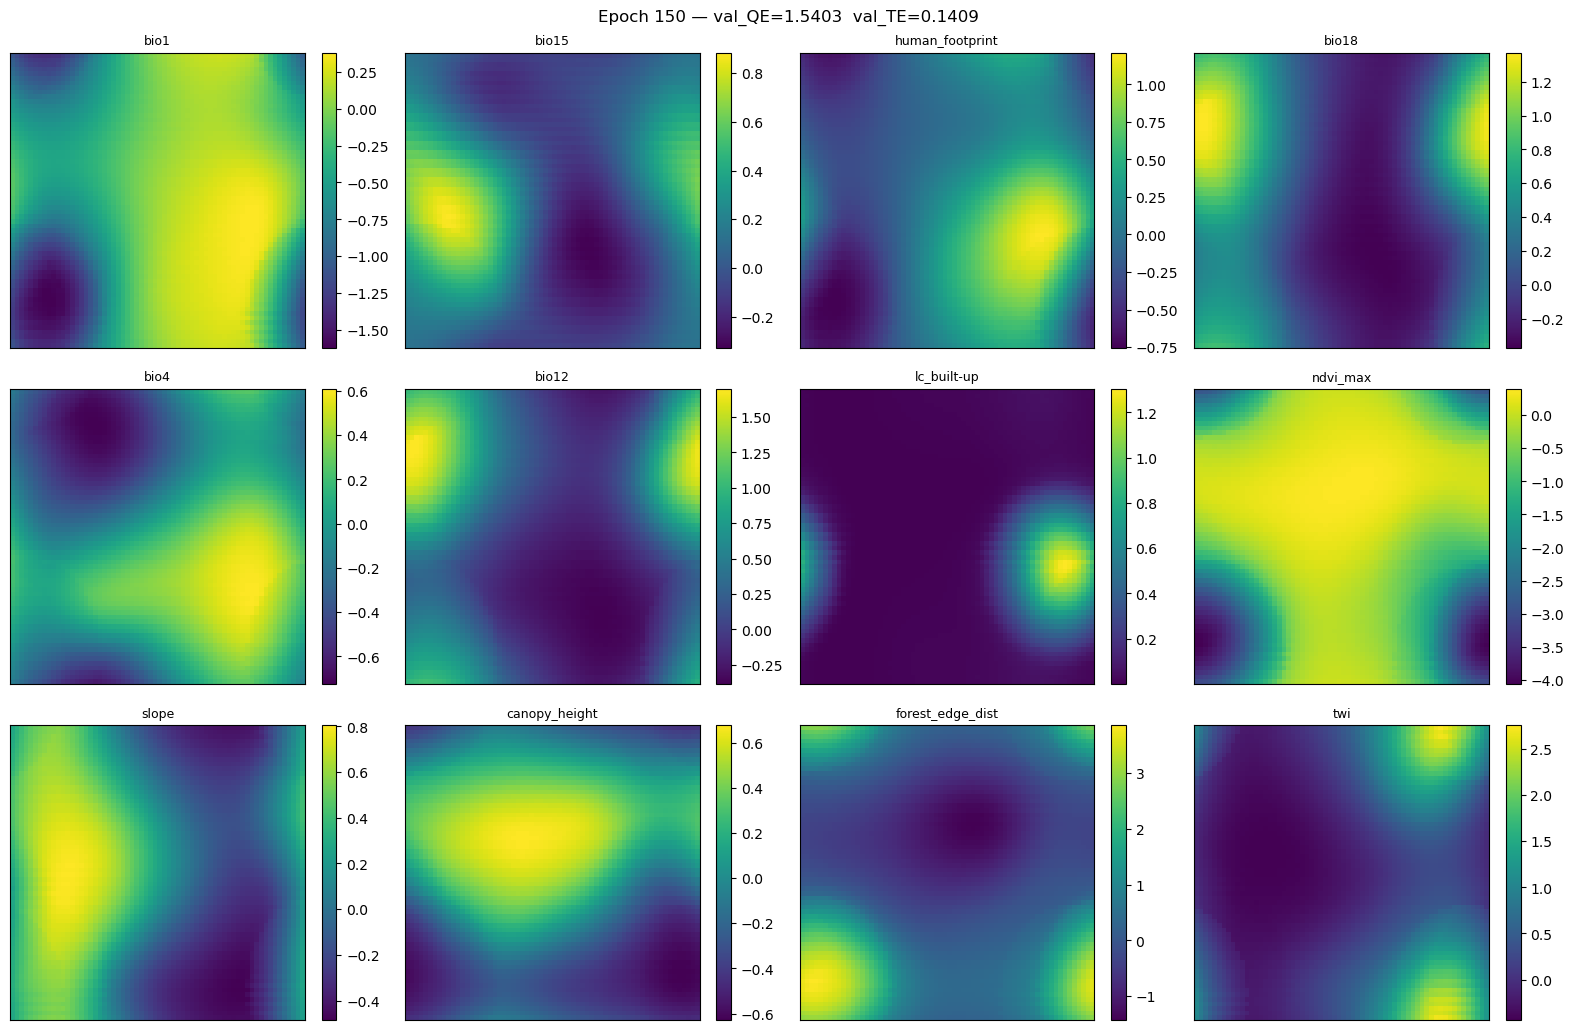
\includegraphics[width=\linewidth]{codebook_epoch_150}
  \medskip
  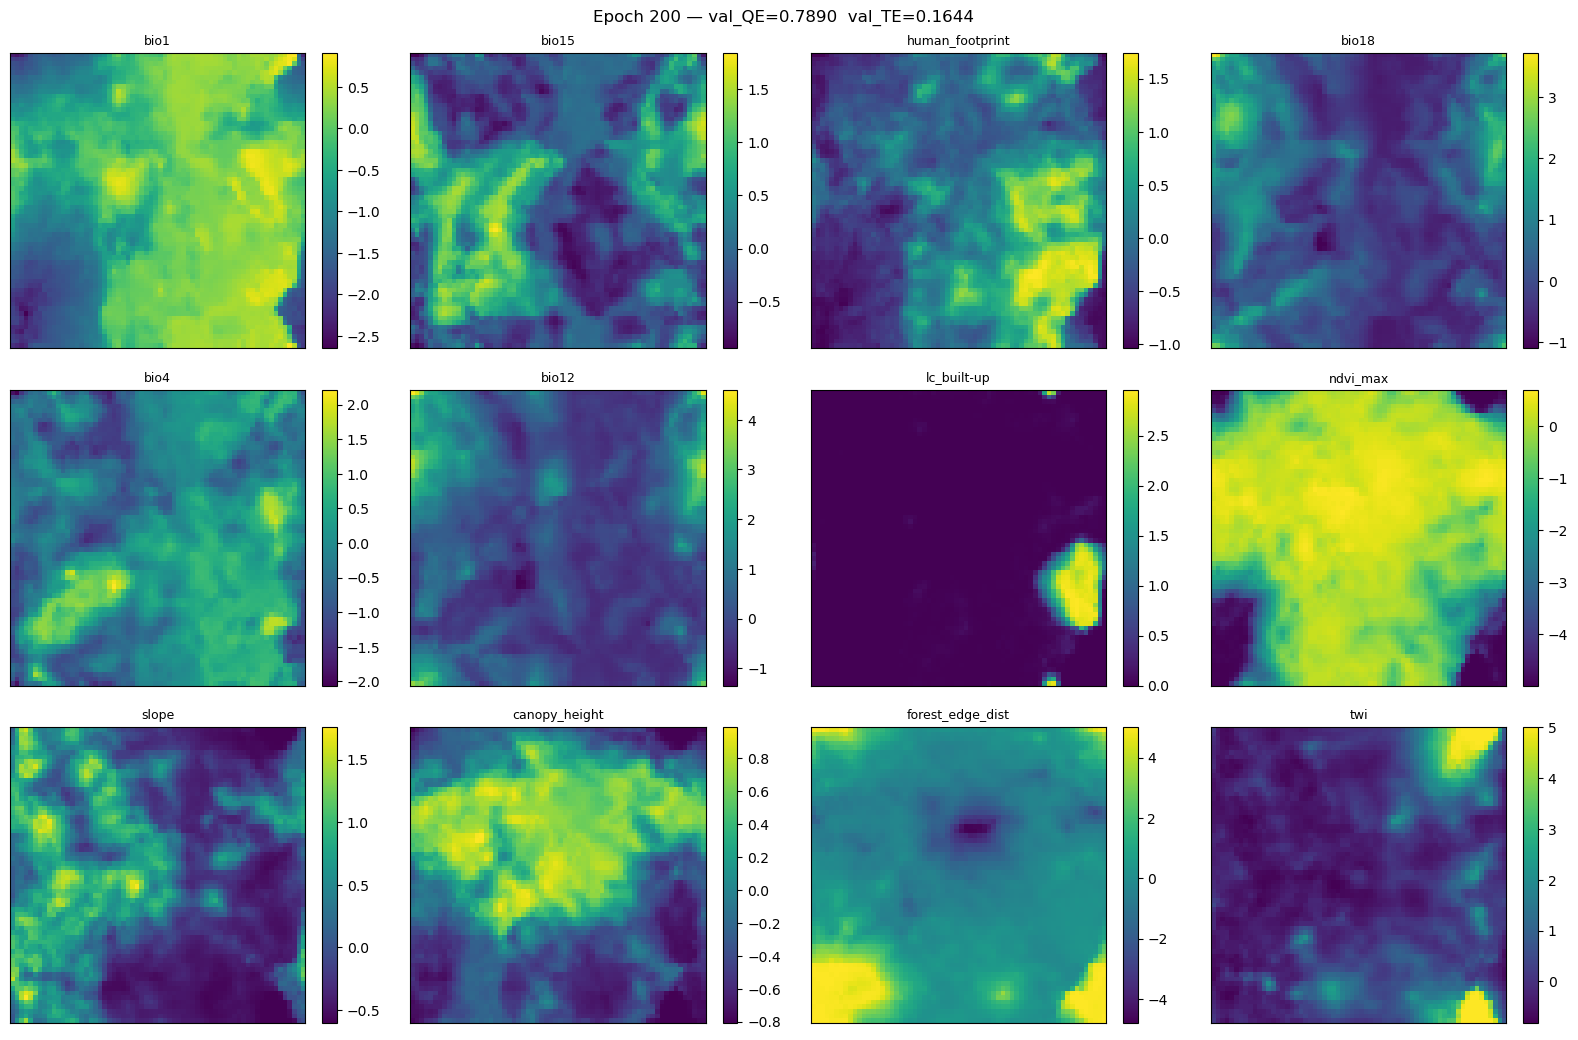
\includegraphics[width=\linewidth]{codebook_epoch_200}
  \caption{SOM codebook feature maps at epoch~150 (top) and
  epoch~200 (bottom). At 150~epochs the codebook shows smooth
  gradients with distinct regional structure across all 12
  features. At 200~epochs, overtraining causes feature maps to
  fragment into noise---particularly visible in slope, TWI, and
  bio15---as the reduced neighbourhood radius allows individual
  neurons to chase local samples rather than preserving global
  topology.}
  \label{fig:codebook-comparison}
\end{figure}

\section{GNN-SDM Training Diagnostics}
\label{app:gnn-training}

\begin{figure}[htbp]
  \centering
  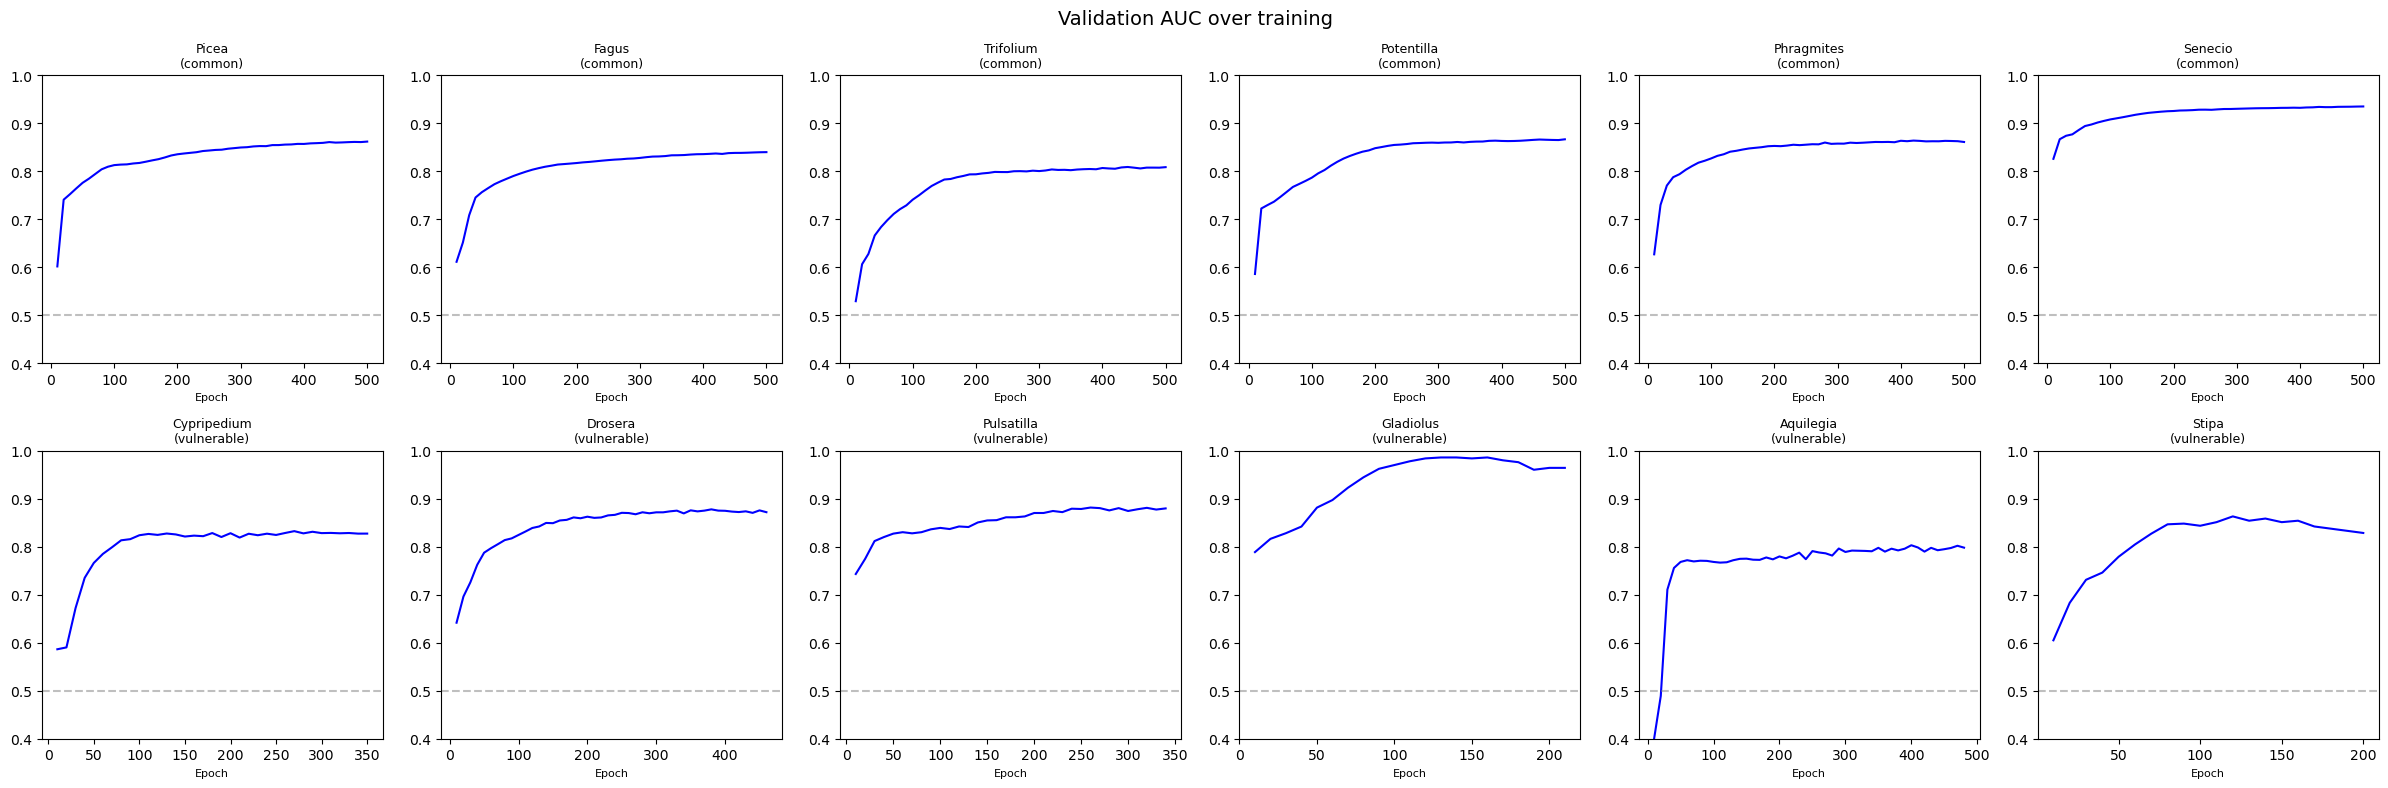
\includegraphics[width=0.85\linewidth]{gnn_training_val}
  \caption{Validation AUC curves during GNN-SDM training for
  the 12 selected species (6~common, 6~vulnerable). Early
  stopping restores the model at peak validation AUC. Most
  species converge within 200--350 epochs; common species with
  more training data tend to use the full 500-epoch budget.}
  \label{fig:gnn-val-auc}
\end{figure}

\begin{figure}[htbp]
  \centering
  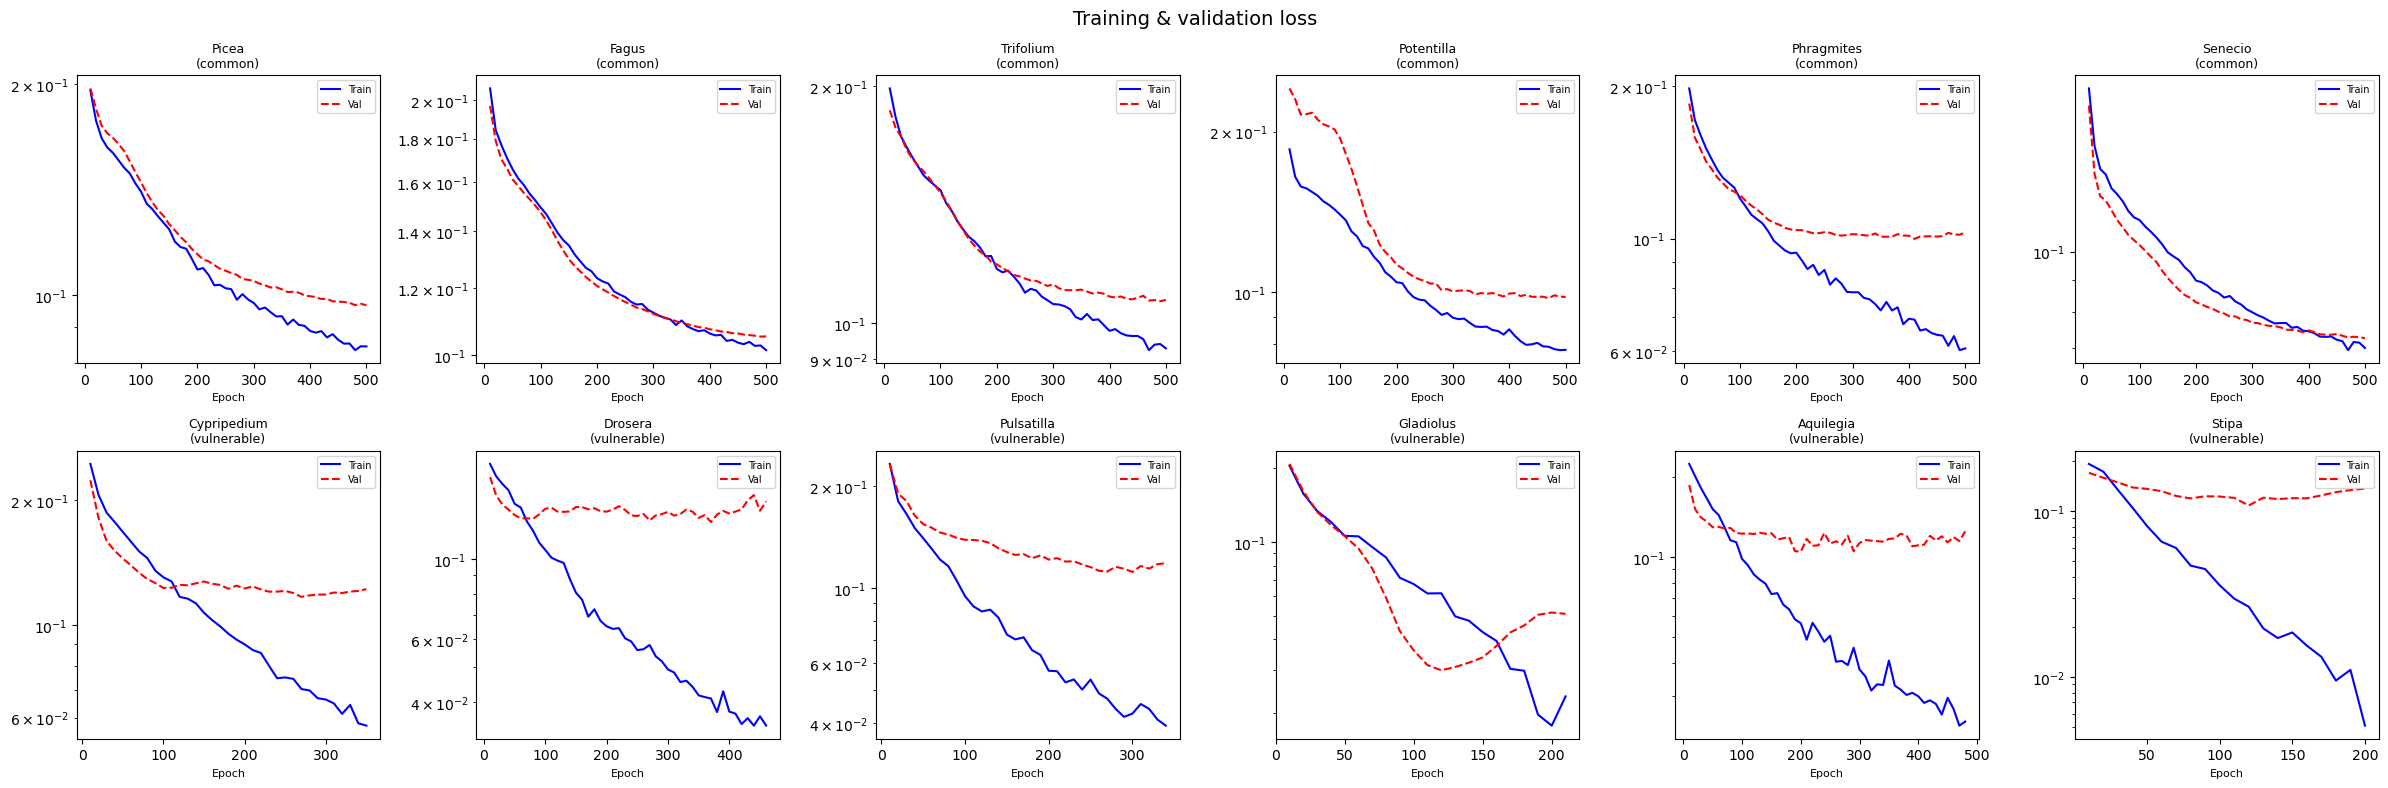
\includegraphics[width=0.85\linewidth]{gnn_training}
  \caption{Training and validation loss (weighted MSE) for the
  12 selected species. The gap between training and validation
  loss remains small throughout, indicating minimal overfitting.
  Dropout ($p = 0.2$) and early stopping provide sufficient
  regularisation.}
  \label{fig:gnn-train-loss}
\end{figure}

\section{Per-Species Habitat Suitability Maps}
\label{app:suitability-maps}

\begin{figure}[htbp]
  \centering
  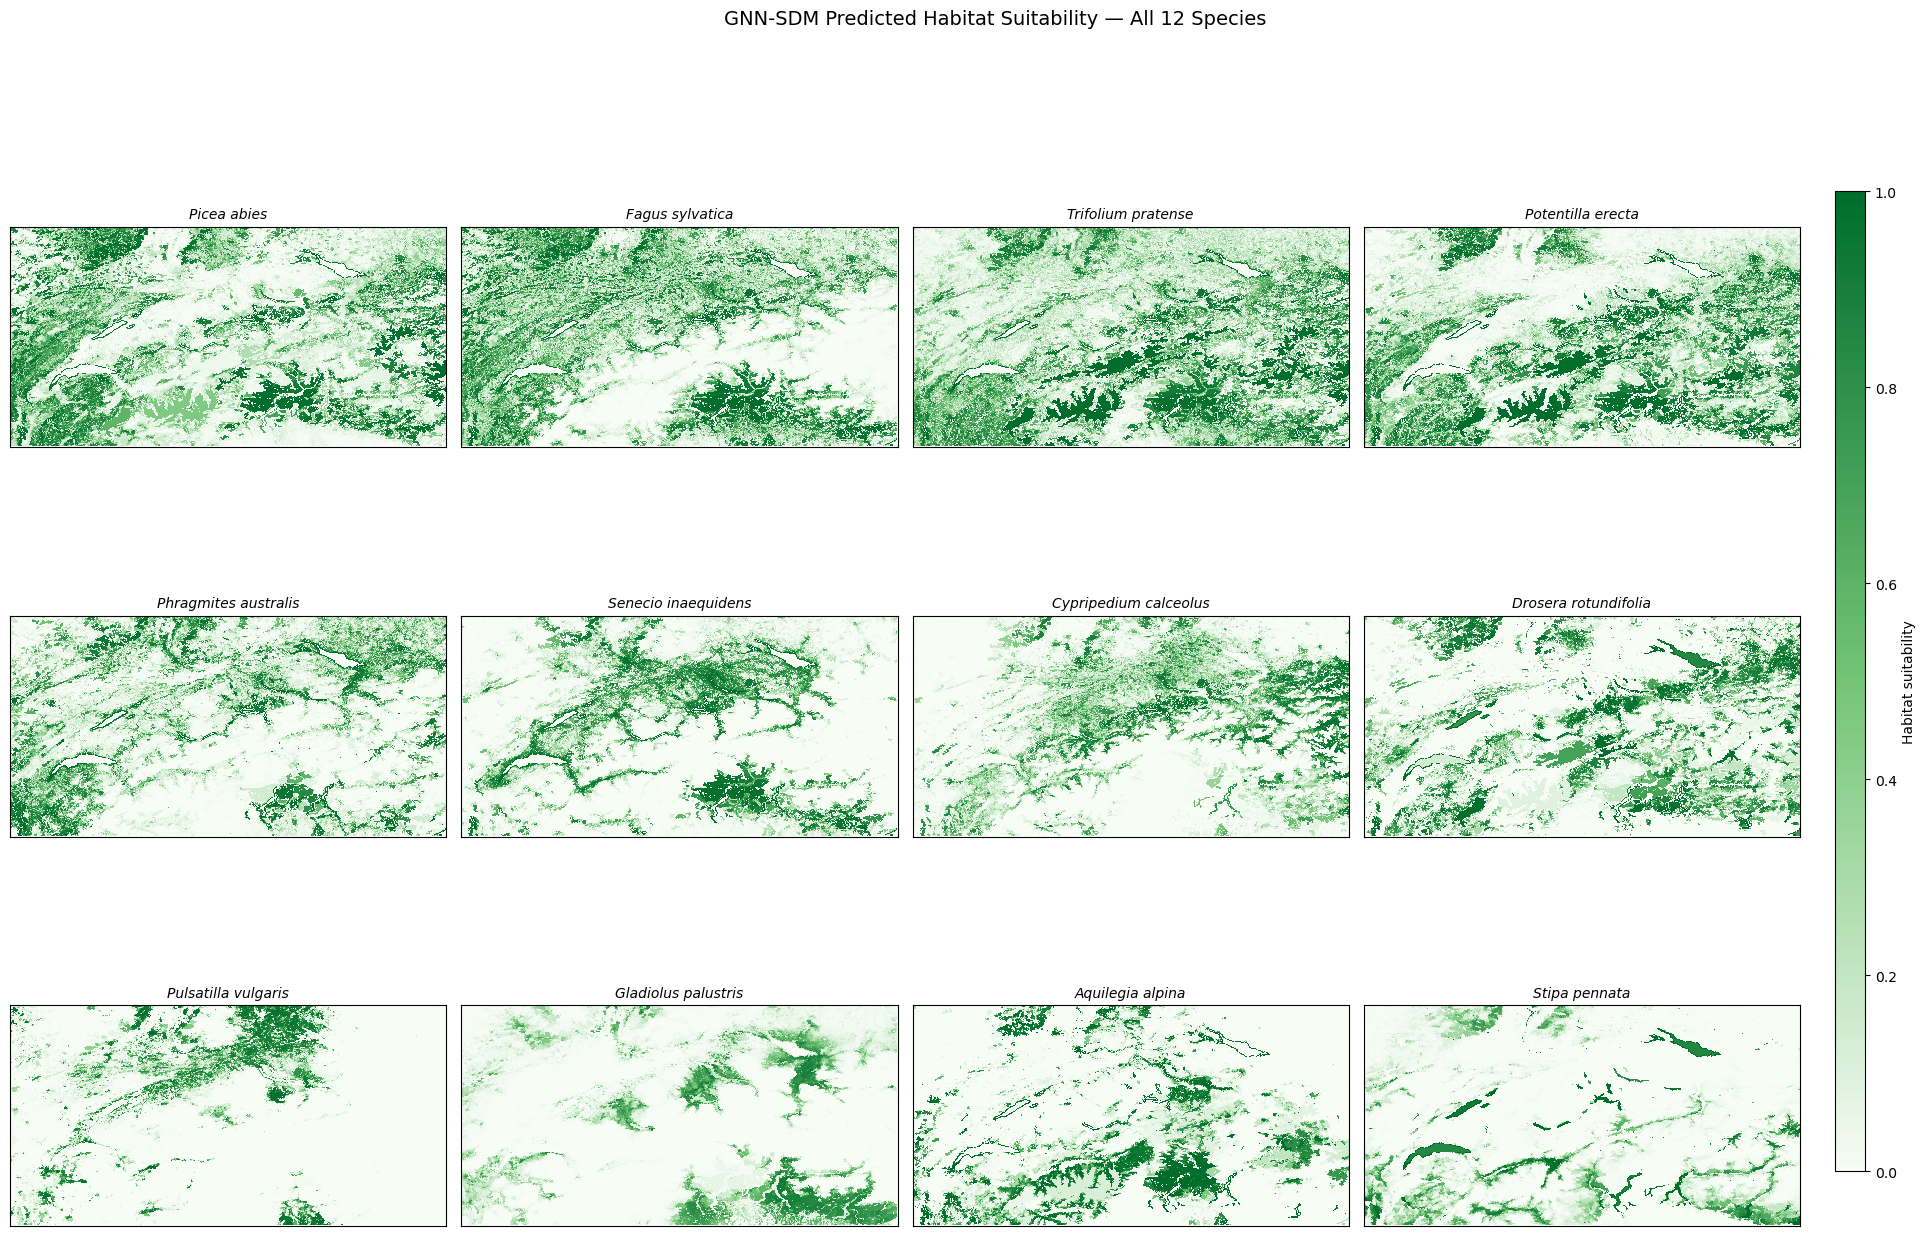
\includegraphics[width=\linewidth]{suitablity_per_species}
  \caption{GNN-SDM habitat suitability maps for the 12 selected
  species. Warm colours indicate high predicted suitability.
  Common species (top two rows) show broader predicted ranges
  consistent with their generalist niches, while vulnerable
  species (bottom two rows) display concentrated suitability
  in restricted habitat patches.}
  \label{fig:suitability-per-species}
\end{figure}


\end{document}
